%\chapter{Output using dynamic textures}
\chapter{Metamaterial Textures}
\label{chapter:textures}

% Digital fabrication machines such as 3D printers excel at producing arbitrary shapes, such as for decorative objects. Recently, researchers proposed going beyond designing merely the external shape, but to divide materials into a large number of cells and to design each cell's structure to perform a specific deformation [27, 33]. Such structures are also known as \textit{metamaterials,} which are ``artificial structures with mechanical properties that are defined by their usually repetitive cell patterns, rather than the material they are made of" [37]. The ability to design each cell individually allows for literally thousands of degrees of freedom.

% Researchers used the concept of metamaterials to design mechanical properties of materials, e.g., vary the stiffness across an object [54], make materials contract in two dimensions when compressed in one dimension [7, 56], damp an impact [55], or change the shape and surface of materials on a macroscopic [6, 35] or microscopic scale [11, 67]. 

We demonstrated in the previous sections that metamaterials can be appropriated to process analog signals in the form of mechanisms and even digital information. While the previous concepts were demonstrated at examples of complete devices featuring input handles, the processing part and an output (e.g., the retracting bolt in the door latch example). However, the focus of our previous works was clearly on processing information and forces.

In this work, we apply the main idea behind metamaterials, i.e., subdivision into a large number of cells and customization on a per-cell basis, to the \textit{outsides} of 3D printed objects. The resulting \textit{metamaterial textures} allow designers to shape how the object interacts with the environment and with the tactile sense of the user.


\section{Overview of metamaterial textures}

Metamaterial textures are 3D printed surface geometries that can perform a controlled transition between two or more textures. Haptic properties, such as compliance \cite{Schumacher2015}, weight, and static texture can enhance 3D objects and are easy to fabricate. More complex fabrication machines, such as multi-material 3D printers, also allow for continuously controllable textures \cite{Guttag2015}. However, so far, they do not apply \textit{objects} and are limited by one texture. 

In this work, we introduce metamaterials that undergo a controlled transformation when an external force is applied, resulting in \textit{multiple} dynamic textures. Figure \ref{fig:1-door-handle-ridges-spiky} shows an example. 

\begin{figure} [h]
    \centering
    %\includegraphics[width=\textwidth]{chapters/metamaterial-textures-FIG/1-door-handle-ridges-spiky.pdf}
    \includegraphics[width=\textwidth]{chapters/introduction-FIG/4-overview-textures.pdf}
    \caption[Short figure name.]{When an external force is applied, metamaterial textures undergo a controlled transformation. This door handle, for example, transforms (a) from flat (b) to rippled (c) to spiky, allowing the person behind the door to set a tactile message with three levels of \textit{enter/busy/do not enter} messages for visually impaired or sighted users trying to enter.
    \label{fig:1-door-handle-ridges-spiky}}
\end{figure}

This door handle transforms from flat to rippled to spiky, allowing the person behind the door to set three levels of \textit{enter/busy/do not enter} tactile messages for everyone trying to enter. For completeness, we integrated our textured handle with our metamaterial door latch (Figure \ref{fig:1 metanism-door latch}).

As shown in Figure \ref{fig:2-door-handle-inside}, the inside of the door handle consists of a grid of cells, which controls how the texture on the object's surface will be formed.

\begin{figure} [h]  
    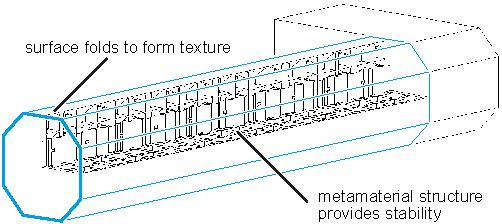
\includegraphics[width=\textwidth]{chapters/metamaterial-textures-FIG/2-door-handle-inside.pdf}
    \caption[Short figure name.]{Metamaterial textures are made from cells that can fold upwards, creating a tactile bump. The metamaterial allows for this behavior while simultaneously providing stability. 
    \label{fig:2-door-handle-inside}}
\end{figure}

Figure \ref{fig:3-door-handle-fold-cell} illustrates the design of the underlying cells, which we call \textit{fold cells.} Each cell implements a simple mechanism that transforms horizontal compression into vertical deformation, i.e., it \textit{folds} upwards when compressed. The cell consists of two four-bars, which is a basic linkage the rigid members of which move in parallel. When the cell is compressed horizontally it causes the four-bars to shear and the cell to fold upwards, creating a tactile bump. Hence, chaining multiple of these cells allows \textit{popping out a texture} on the surface of the object. These four-bars can be repeated inside the object until it is filled.

\begin{figure} [h]  
    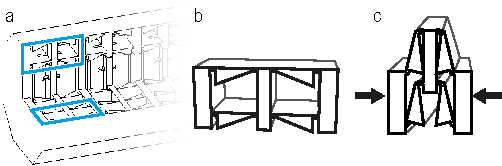
\includegraphics[width=\textwidth]{chapters/metamaterial-textures-FIG/3-door-handle-fold-cell.pdf}
    \caption[Short figure name.]{(a) Textured objects consist of many (b) unit cells, which (c) pop out of the object's surface, when compressed. 
    \label{fig:3-door-handle-fold-cell}}
\end{figure}

Metamaterial textures are generally actuated to transition between textures by a global compression. To ease user interaction, we deploy them with a mechanism that allows producing the force required to deform the metamaterial texture. Figure \ref{fig:4-strings-in-door-handle} shows the mechanism we use to actuate the door handle texture in Figure \ref{fig:1-door-handle-ridges-spiky}. The mechanism runs strings through the door handle. As the user turns the knob, the strings are wound up and cause all fold cells to compress and to fold outward, forming the texture. During actuation metamaterial textures compress by a certain amount---30\% in the case of the door handle example in Figure \ref{fig:1-door-handle-ridges-spiky}. This means our approach is limited to objects for which length is not a critical property. 

\begin{figure} [h]  
    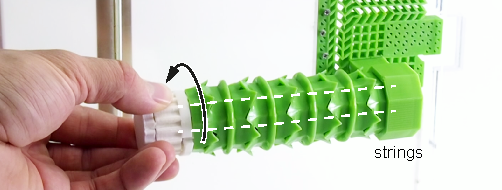
\includegraphics[width=\textwidth]{chapters/metamaterial-textures-FIG/4-strings-in-door-handle.pdf}
    \caption[Short figure name.]{Users transition through the door handle’s embedded textures by turning the knob. That winds up the strings on the inside, which compresses all cells and forms the textures.
    \label{fig:4-strings-in-door-handle}}
\end{figure}


\subsubsection{Application examples}

Metamaterial textures are suitable for conveying tactile messages or providing tactile feedback, for rapid prototyping of textured objects, or for adapting objects on demand. 

\textit{Conveying tactile messages. } 
Figure \ref{fig:1-door-handle-ridges-spiky} showed an example for this category as a door handle that utilizes its surface to inform users (visually impaired or sighted) about one’s availability for interruptions. We achieve three textures within the one object by (1) alternating the two textures row-wise and (2) defining the sequence in which they pop out based on the amount of compression, i.e., compressing the door handle halfway only activates the smoother ridges, and compressing it all the way adds the spiky texture to the previous bumpy texture. 

\textit{Adapting the functionality of an object to the context of use. }
Figure \ref{fig:5-shoe-sole} shows a shoe sole with a metamaterial texture. It can be transformed from a flat sole to a corrugated one for more traction on snow or mud. This example illustrates one benefit of these metamaterial structures: they add enough \textit{stability} to the origami-like surface to hold the weight of an adult (here 55 kg). To achieve this, we designed our cell to fold tightly, which prevents the beams from buckling in order to maximize strength (Figure \ref{fig:3-door-handle-fold-cell}c). 

\begin{figure} [!h]  
    \includegraphics[width=\textwidth]{chapters/metamaterial-textures-FIG/5-shoe-sole.pdf}
    \caption[Short figure name.]{(a) This shoe sole is flat by default. (b) The user transforms it into a treaded sole it by pulling a string, e.g., when it starts snowing. (c) Note that the sole is functional and robust enough to walk on.
    \label{fig:5-shoe-sole}}
\end{figure}

\textit{Exploring texture designs quickly. }
One of the qualities of metamaterial textures is that they can be continuously actuated to different levels (Figure \ref{fig:6-bike-grip}a-c). This is useful when trying to explore how ``strong" a texture should be during rapid prototyping. To test for the ergonomics of this bicycle grip, designers can prevent cells locally from folding. Figure \ref{fig:6-bike-grip}d shows that sliding spacers into the material causes those cells to resist the compression. Designers can then again explore if the design feels right (Figure \ref{fig:6-bike-grip}e). 

\begin{figure} [!h]  
    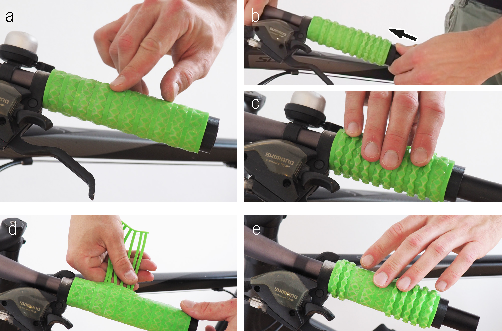
\includegraphics[width=\textwidth]{chapters/metamaterial-textures-FIG/6-bike-grip.pdf}
    \caption[Short figure name.]{(a) Designers fabricate one single bicycle grip that they (b) actuate continuously to different levels, (c) to feel the tactile qualities during rapid prototyping. (d) By inserting spacers after fabrication that (e) deactivates selected rows allows them to further investigate the grip’s ergonomics.
    \label{fig:6-bike-grip}}
\end{figure}

Metamaterial textures allow product designers to quickly iterate through multiple textures in one 3D print only, instead of fabricating many prototypes, which is slow. In fact, designers and researchers agree that tactile designs ``need to be felt early and often" \cite{Schneider2017}. Similar approaches exist for quickly iterating over rigid 3D shapes \cite{Mueller2014a}, we extend this idea to texture prototyping. 


\section{Contributions}
Our main contribution is the concept of embedding \textit{multiple} dynamic textures into one 3D printed object using metamaterials. Such textured objects allow for continuously transitioning between magnitudes of the texture. Furthermore, they allow users to define the sequence in which the cells fold, which enables transitioning between multiple integrated textures after fabrication. 

Our textures are integrated in the object at printing time. We contribute parameterized metamaterial cells that function using a single material and that enable a range of textures by only varying the cell geometry. 

To assist users and researchers in designing new textures using metamaterials, we contribute an interactive editor that features a fast preview of the texture transformation.


\section{Design space of metamaterial textures}

To summarize the capabilities of metamaterial textures, we characterize their design space, as illustrated in Figure \ref{fig:7-design-space}. The resulting design space consists of six dimensions:

\begin{figure} [h]  
    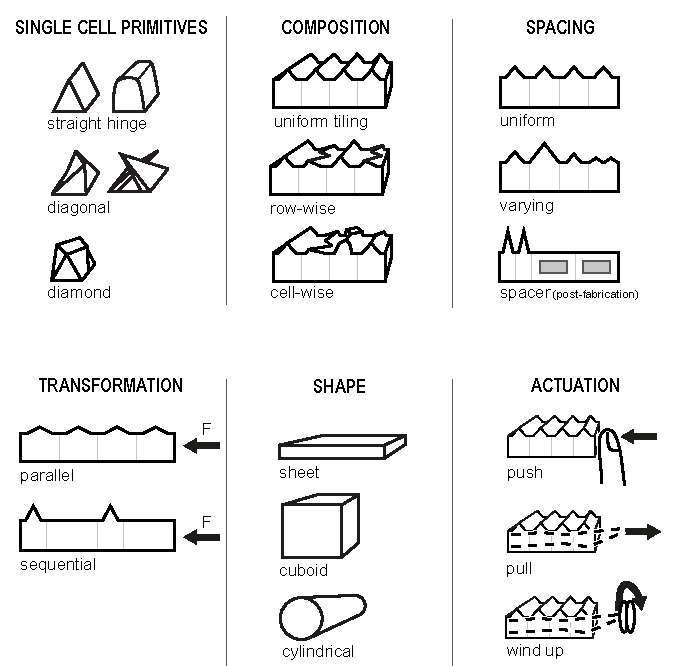
\includegraphics[width=\textwidth]{chapters/metamaterial-textures-FIG/7-design-space.pdf}
    \caption[Short figure name.]{Our six-dimensional design space describing metamaterial textures.
    \label{fig:7-design-space}}
\end{figure}

\paragraph{Single cell primitives.} We identified three geometry classes that can be parameterized to create a range of shapes for the tactile bump on a single cell: simple straight ridges (which can create box-like cells or rounded cells), diagonal (zigzag, spiky, etc.) or diamond shaped.

\paragraph{Composition.} Single cell primitives can be composed to form a texture by (1) \textit{uniformly tiling} the same cells one next to the other. A more expressive composition can be achieved by (2) chaining cells of the same type \textit{row-wise} (such as in our door handle example). Lastly, it is also possible to (3) compose the texture from a \textit{cell-wise} arrangement, the only restriction being that the positions of the folding hinge must join continuously from one cell to the next in the row.

\paragraph{Spacing.} We identified three possible variations for how to define the space between tactile bumps. The simplest configuration available to designers is to spread out their bumps at equally distant points by \textit{uniformly} spacing cells. To \textit{vary} the spacing between tactile bumps, designers can choose cell parameters which increase or decrease the spacing and chain these cells. A complete explanation of the cell parameters is given in Section \ref{section:amplitude-textures}. Lastly, the distance between bumps can be increased by inserting \textit{spacers} into the material after it was fabricated, which prevents the selected cells from folding. 

\paragraph{Transformation.} Designers can define how the transformation between textures will be performed: the texture can fold in parallel, sequentially, or a combination of these. A parallel transformation implies that all cells fold at once (e.g., the bike grip example). A sequential transformation causes cells to fold subsequently as the force increases, as illustrated by the door handle in Figure \ref{fig:1-door-handle-ridges-spiky}. This is detailed in Section \ref{section:force-dependent-textures}.

\paragraph{Shape.} We identified three shape classes that our metamaterial textures can cover. The simplest shape that metamaterial textures can be applied to is a planar sheet. It can also be applied to cylindrical shapes (e.g., bike grip) or on the outside of cuboid shapes, e.g., the door handle example. 

\paragraph{Actuation.} Since our textures are actuated by global compression, we see three actuation possibilities for our resulting textures. The simplest form of actuating metamaterial textures is by pushing them manually to compress. Alternatively, designers can run strings through the material that are either pulled or wound up. While in this paper we explore the idea of having no electronics in our materials and use human actuation for all three actuation classes, using motors or other automated actuators is certainly possible.


\section{Implementing textures based on cells}

Our materials consist of cells on a regular grid. In the following, we describe the design of the cells. In order to create different textures, we describe the cell parameters that can be varied by designers and their effects. For simplicity, we first describe the mechanics of the fold cell at the example of creating a simple bumpy structure. Then, we focus on the top of the cell and how to create more complex texture geometries.

Our prototypes were printed using \textit{NinjaFlex,} a rubber-like filament, on an \textit{Ultimaker 2+,} which is a consumer-level fused deposition modeling (FDM) 3D printer. The fold cells have a width of $15\, \mathrm{mm}$ and a height and depth of $7.5\, \mathrm{mm}$. 


\subsection{Geometry of the fold cell}

Figure \ref{fig:8-basic-texture-cell} illustrates the structure of our unitary cell, the fold cell. It consists of two walls that are connected to four members by living hinges, i.e., thin parts that, due to their reduced stiffness, can flex.

Compressing the cell causes the internal four-bars to shear in a pre-defined direction, here it shears upwards. The shearing direction is encoded into the triangular shape of the members (Figure \ref{fig:8-basic-texture-cell}c): having the thicker part of the members towards the walls prevents them from tilting down as they would collide with the walls; reversing the triangular members would result in a downwards fold.

\begin{figure} [h]  
    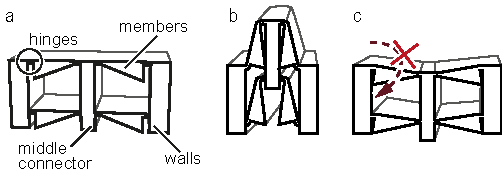
\includegraphics[width=\textwidth]{chapters/metamaterial-textures-FIG/8-basic-texture-cell.pdf}
    \caption[Short figure name.]{The fold cell consists of parametrizable walls, hinges and members that enable a stable fold to transform the material from straight to textured (here corrugated).
    \label{fig:8-basic-texture-cell}}
\end{figure}


\subsection{Amplitude and frequency of a texture}
\label{section:amplitude-textures}

The height of the protruding texture is defined by the length of the fold cell’s members. As shown in Figure \ref{fig:9-amplitude-frequency}a, longer members allow the resulting texture to pop out more from the 3D object. We call this the amplitude of the texture.

We found the relationship of maximum amplitude and member length to be described as:

\[
    amplitude_{max} = \sqrt{\left(\frac{c}{2}-w-m \right)^2 - t^2}
\]

where $c$ denotes the cell width, $w$ the wall thickness, $m$ the middle connector thickness, and $t$ the member thickness.

While an increased wall thickness decreases the amplitude, it simultaneously decreases the \textit{frequency} of the texture. Figure \ref{fig:9-amplitude-frequency}b illustrates how increasing the wall thickness of the cells separates neighboring cells further apart and thus reduces the resulting texture’s frequency. To achieve a high frequency with low amplitude, we can split the cell in two, as shown in Figure \ref{fig:9-amplitude-frequency}c.

The same parameters that influence the amplitude also define the maximum compression ratio of the texture. For example, cells with thick walls can be compressed by a smaller extend than cells with thin walls. The compression ratio per cell is therefore modeled as

\[
    compression_{cell} = \frac{2w + 2t + m}{c}.
\]


\begin{figure} [h]  
    \includegraphics[width=\textwidth]{chapters/metamaterial-textures-FIG/9-amplitude-frequency.pdf}
    \caption[Short figure name.]{(a-b) The length of the fold cell’s members defines the texture’s amplitude, i.e., the height of each bump. (c) The amplitude can be varied across the material and cells can be split to create a higher frequency.
    \label{fig:9-amplitude-frequency}}
\end{figure}


\subsection{Force-dependent textures}
\label{section:force-dependent-textures}

The thickness of the hinges defines how much force is required to fold them outwards. Figure \ref{fig:10-force-dependent-cells} illustrates that because thicker hinges require more force to be deformed than thin hinges (in fact, the required force is to the power of three \cite{Gross2014}), they also \textit{fold later} as they are subjected to constant compression. 

To embed multiple textures in one object, as demonstrated in our door handle example shown in Figure \ref{fig:1-door-handle-ridges-spiky}, designers specify a smaller hinge thickness for the cells that will pop up first (cf. the ridges in the door handle) and a larger hinge thickness for the cells that will fold later (cf. the spiky cells). This allows designers to potentially make every row dependent on different amounts of force to create animated textures on 3D objects. 

\begin{figure} [h]  
    \includegraphics[width=\textwidth]{chapters/metamaterial-textures-FIG/10-force-dependent-cells.pdf}
    \caption[Short figure name.]{(a) Here, we demonstrate how our approach embeds multiple textures in one surface by varying the thickness of the hinges. (b) The upper cell’s hinges are thinner and thus fold before (i.e., under less force) than the lower cell’s hinges, which are 50\% thicker. (c) If the hinge thickness is uniform across cells, they fold simultaneously under the same load.
    \label{fig:10-force-dependent-cells}}
\end{figure}

While a more exhaustive technical evaluation is planned for future work, we report a simple experiment to evaluate an example structure, featuring a row with four different fold cells. Each cell in Figure \ref{fig:11-force-test} has a unique hinge thickness; from left to right  $0.6\, \mathrm{mm}$,  $0.8\, \mathrm{mm}$,  $0.4\, \mathrm{mm}$,  $1.0\, \mathrm{mm}$. Figure \ref{fig:11-force-test}a shows the third cell folding upwards as the whole row is compressed while connected to a force gauge. As expected, we confirmed that the folding order of our printed cells is indeed dictated by their increasing hinge thickness:  $0.4\, \mathrm{mm}$ folds at  $3.0\, \mathrm{N}$,  $0.6\, \mathrm{mm}$ folds at $3.65\, \mathrm{N}$, $0.8\, \mathrm{mm}$ folds at $6.4\, \mathrm{N}$ and $1.0\, \mathrm{mm}$ folds at $8.15\, \mathrm{N}$. 

\begin{figure} [h]  
    \includegraphics[width=\textwidth]{chapters/metamaterial-textures-FIG/11-force-test.pdf}
    \caption[Short figure name.]{Our force test confirms that by varying the hinge thicknesses, we can control when the cell folds up.
    \label{fig:11-force-test}}
\end{figure}


\subsection{Single cell primitives}

We now describe how to create bumps with more expressive shapes. So far, we have seen only textures created by bumps with a triangular protrusion. Now, we demonstrate that by simply altering the hinges on the top of the single cells, we can achieve more interesting results. 

\subsubsection{Triangular, squared and rounded texture bumps}

The simplest bump is just a straight fold, which resembles a small triangle (Figure \ref{fig:12-straight-hinges}a). Next, we design a box-like texture bump by specifying equal widths for all members (Figure \ref{fig:12-straight-hinges}b). We can also create round bumps (Figure \ref{fig:12-straight-hinges}c) by making the hinge in the middle long and double its thickness (here to $0.8\, \mathrm{mm}$).

\begin{figure} [h]  
    \includegraphics[width=\textwidth]{chapters/metamaterial-textures-FIG/12-straight-hinges.pdf}
    \caption[Short figure name.]{Variations of textures using a straight fold: (a) triangular folds, (b) box-like or (c) round bumps.
    \label{fig:12-straight-hinges}}
\end{figure}

\subsubsection{Zigzag texture bumps}
The simple straight bend that we demonstrated can be transformed to create more elaborate textures. We do so by offsetting the hinge positions on both edges of the cell, as illustrated by Figure \ref{fig:13-diagonal-explained}a. This results in a diagonal folding up. The connection to the cell's middle connector is only possible at a small part in the middle of the hinge, which requires the connector to be tapered in the z-axis (Figure \ref{fig:13-diagonal-explained}b). Despite de connection being very small, the structure works as before because the lower members push the cell up. 

Note that the diagonal hinge also reduces the maximum amplitude and the compression ratio. This is because the offset of the hinge created members of different lengths, i.e., a shorter and a longer member. The cell can now only fold up to the extent of the shorter member.

\begin{figure} [h]  
    \includegraphics[width=\textwidth]{chapters/metamaterial-textures-FIG/13-diagonal-explained.pdf}
    \caption[Short figure name.]{(a) Adding horizontal offsets to the hinge creates diagonal folds. (b) The connector width to the lower cell structure needs to be decreased gradually to connect to the cell top. (c) Composing multiple diagonal fold cells creates zigzag patterns that (d) can be varied in magnitude.
    \label{fig:13-diagonal-explained}}
\end{figure}

\subsubsection{Spiky texture bumps}
To create the spiky texture from our door handle example, we take the zigzag pattern from Figure \ref{fig:13-diagonal-explained}a and remove the material from the hinge, only leaving a thin connection in the middle as shown in Figure \ref{fig:14-spiky-patterns}a. This results a malleable spiky texture as the triangles fold upwards but are disconnected from their walls.

\begin{figure} [!h]  
    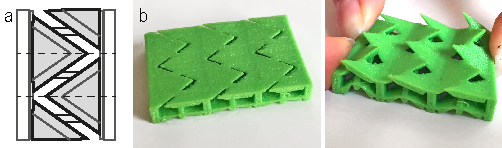
\includegraphics[width=\textwidth]{chapters/metamaterial-textures-FIG/14-spiky-patterns.pdf}
    \caption[Short figure name.]{(a) Leaving gaps between the members of the cell top (b) allows for creating spiky textures.
    \label{fig:14-spiky-patterns}}
\end{figure}

\subsubsection{Diamond texture bumps}
The diamond bump can be created by changing the location where the horizontal offset is effective in the vertical axis. Figure \ref{fig:15-diamond-patterns} shows how this allows designers to create a Y-shaped pattern, which has the effect of flattening out in the middle. By mirroring this pattern to the neighbor cell, it creates a diamond-shaped texture. It is also possible to achieve the diamond pattern on a single cell, by varying the vertical offsets on both sides (Figure \ref{fig:15-diamond-patterns}b).

\begin{figure} [h]  
    \includegraphics[width=\textwidth]{chapters/metamaterial-textures-FIG/15-diamond-patterns.pdf}
    \caption[Short figure name.]{(a-b) Offsetting the hinge vertically and horizontally creates (c) diamond shaped textures, which flatten in the middle and thus create a different tactile feel.
    \label{fig:15-diamond-patterns}}
\end{figure}


% \section{Interactive Editor for Textures}

% Figure \ref{fig:16-editor-ui} shows the interactive editor we built to assist designers in creating textures based on metamaterials. Here, we see a user creating a block that when pushed displays a zigzag texture on the top. 

% \begin{figure} [h]  
%     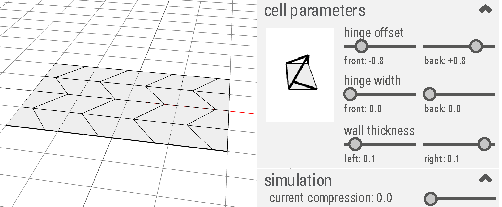
\includegraphics[width=\textwidth]{chapters/metamaterial-textures-FIG/16-editor-ui.pdf}
%     \caption[Short figure name.]{Our editor assists users in creating metamaterial textures. Users adjust the cell geometry using sliders and lay the cells out on the grid.
%     \label{fig:16-editor-ui}}
% \end{figure}


% \subsection{User interaction}

% In the interactive editor, we exploit the fact that the fold cell is fully parameterized. Users can set all parameters (Figure \ref{fig:16-editor-ui}, \textit{right}), for example hinge offset, width and wall thickness, simply by dragging the individual sliders. An interactive preview of a cell in its actuated state (Figure \ref{fig:16-editor-ui}, \textit{left from the parameters}) allows users to see how the cell will look like once placed and actuated. After setting all parameters, users can arrange the cells on a regular grid to create textures from metamaterials. 


% \subsection{Previewing textures by means of simulation}

% The editor offers a preview of the resulting texture based on the user's current metamaterial design. They can interactively preview the different textures, which result from different compression rates by simply dragging the slider (Figure \ref{fig:17-editor-simulation}) that specifies the current compression. The deformation of the textures is rendered in real-time.

% \begin{figure} [h]  
%     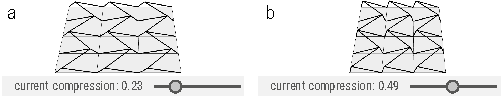
\includegraphics[width=\textwidth]{chapters/metamaterial-textures-FIG/17-editor-simulation.pdf}
%     \caption[Short figure name.]{Users interactively preview their textures by dragging the slider that sets the simulated compression. 
%     \label{fig:17-editor-simulation}}
% \end{figure}


% \subsection{Software implementation}

% Our editor runs in a browser. It is based on the editor for metamaterial mechanisms [15], which is built using node.js (a Javascript runtime framework) and utilizes the three.js library for rendering. 

% The simple kinematic simulation that we implemented in our editor allows for previewing, in real-time, how the designed textures fold up when the material is compressed via a GUI slider. Our simulation calculates only geometric transformations by simple propagation, i.e., as a cell compresses, its members move, in turn, these members move the neighboring cell's members, and so forth. 

% Note that at this stage our simulation does not take material properties into account. We opted for this approach as it allows for an interactive simulation (at 30 fps) compared to, e.g., finite element analysis, which is computationally more expensive and therefore slower, but more accurate. 


% \subsection{Generating a printable file}

% To simplify the process of creating a texture based on metamaterials, our editor only requires users to choose how the surface of the cell should fold to form their texture. In fact, the remainder of the 3D object, e.g., its internal structure beyond the top layer, is generated by our editor when users export the final texture. 

% We derive the parameters for the remainder cell geometry from the user defined hinge positions. The wall thickness is derived from the hinge offsets. For a diagonal hinge, we gradually decrease the thickness of the middle connector towards the top so that it connects only to the center of the texture geometry with minimum widths of $0.3\, \mathrm{mm}$. After having created the cell body for the fold cell, we repeat this structure until the user-defined volume is filled. Finally, this geometry is exported into a 3D printable .stl file.


% \subsection{Limitations of the interactive editor}

% Our editor only allows creating objects with simple geometries, i.e., planar, curved, and cylindrical. Our current kinematic simulation enables real-time interaction at the expense of offering more simplistic results. These, however, preview all the textures we demonstrated correctly. 


\section{Editing metamaterial textures}

Figure \ref{fig:16-editor-ui} shows the interactive editor we built to assist designers in creating textures based on metamaterials. Here, we see a user creating a block that when pushed displays a zigzag texture on the top. 

\begin{figure} [h]  
    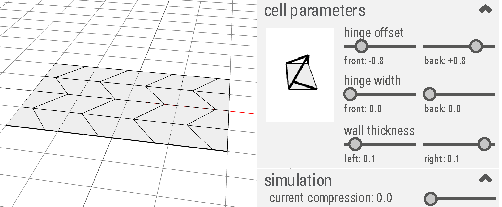
\includegraphics[width=\textwidth]{chapters/metamaterial-textures-FIG/16-editor-ui.pdf}
    \caption[Short figure name.]{Our editor assists users in creating metamaterial textures. Users adjust the cell geometry using sliders and lay the cells out on the grid.
    \label{fig:16-editor-ui}}
\end{figure}


\subsection{User interaction}

In the interactive editor, we exploit the fact that the fold cell is fully parameterized. Users can set all parameters (Figure \ref{fig:16-editor-ui}, \textit{right}), for example hinge offset, width and wall thickness, simply by dragging the individual sliders. An interactive preview of a cell in its actuated state (Figure \ref{fig:16-editor-ui}, \textit{left from the parameters}) allows users to see how the cell will look like once placed and actuated. After setting all parameters, users can arrange the cells on a regular grid to create textures from metamaterials. 

Our editor runs in a browser. It is based on the editor for metamaterial mechanisms, which is built using node.js (a Javascript runtime framework) and utilizes the three.js library for rendering. 

\subsection{Previewing textures by means of simulation}

The editor offers a preview of the resulting texture based on the user's current metamaterial design. They can interactively preview the different textures, which result from different compression rates by simply dragging the slider (Figure \ref{fig:17-editor-simulation}) that specifies the current compression. The deformation of the textures is rendered in real-time.

\begin{figure} [h]  
    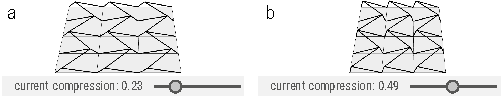
\includegraphics[width=\textwidth]{chapters/metamaterial-textures-FIG/17-editor-simulation.pdf}
    \caption[Short figure name.]{Users interactively preview their textures by dragging the slider that sets the simulated compression. 
    \label{fig:17-editor-simulation}}
\end{figure}

The simple kinematic simulation that we implemented in our editor allows for previewing, in real-time, how the designed textures fold up when the material is compressed via a GUI slider. Our simulation calculates only geometric transformations by simple propagation, i.e., as a cell compresses, its members move, in turn, these members move the neighboring cell's members, and so forth. 

Note that at this stage our simulation does not take material properties into account. We opted for this approach as it allows for an interactive simulation (at 30 fps) compared to, e.g., finite element analysis, which is computationally more expensive and therefore slower, but more accurate. 


\subsection{Generating a printable file}

To simplify the process of creating a texture based on metamaterials, our editor only requires users to choose how the surface of the cell should fold to form their texture. In fact, the remainder of the 3D object, e.g., its internal structure beyond the top layer, is generated by our editor when users export the final texture. 

We derive the parameters for the remainder cell geometry from the user defined hinge positions. The wall thickness is derived from the hinge offsets. For a diagonal hinge, we gradually decrease the thickness of the middle connector towards the top so that it connects only to the center of the texture geometry with minimum widths of $0.3\, \mathrm{mm}$. After having created the cell body for the fold cell, we repeat this structure until the user-defined volume is filled. Finally, this geometry is exported into a 3D printable .stl file.


\subsection{Limitations of the interactive editor}

Our editor only allows creating objects with simple geometries, i.e., planar, curved, and cylindrical. Our current kinematic simulation enables real-time interaction at the expense of offering more simplistic results. These, however, preview all the textures we demonstrated correctly. 




\section{Discussion}

In the following we present a discussion of our prototype centered on its limitations and potential implications (illustrated by Figure \ref{fig:18-discussion}). 

\begin{figure} [h]  
    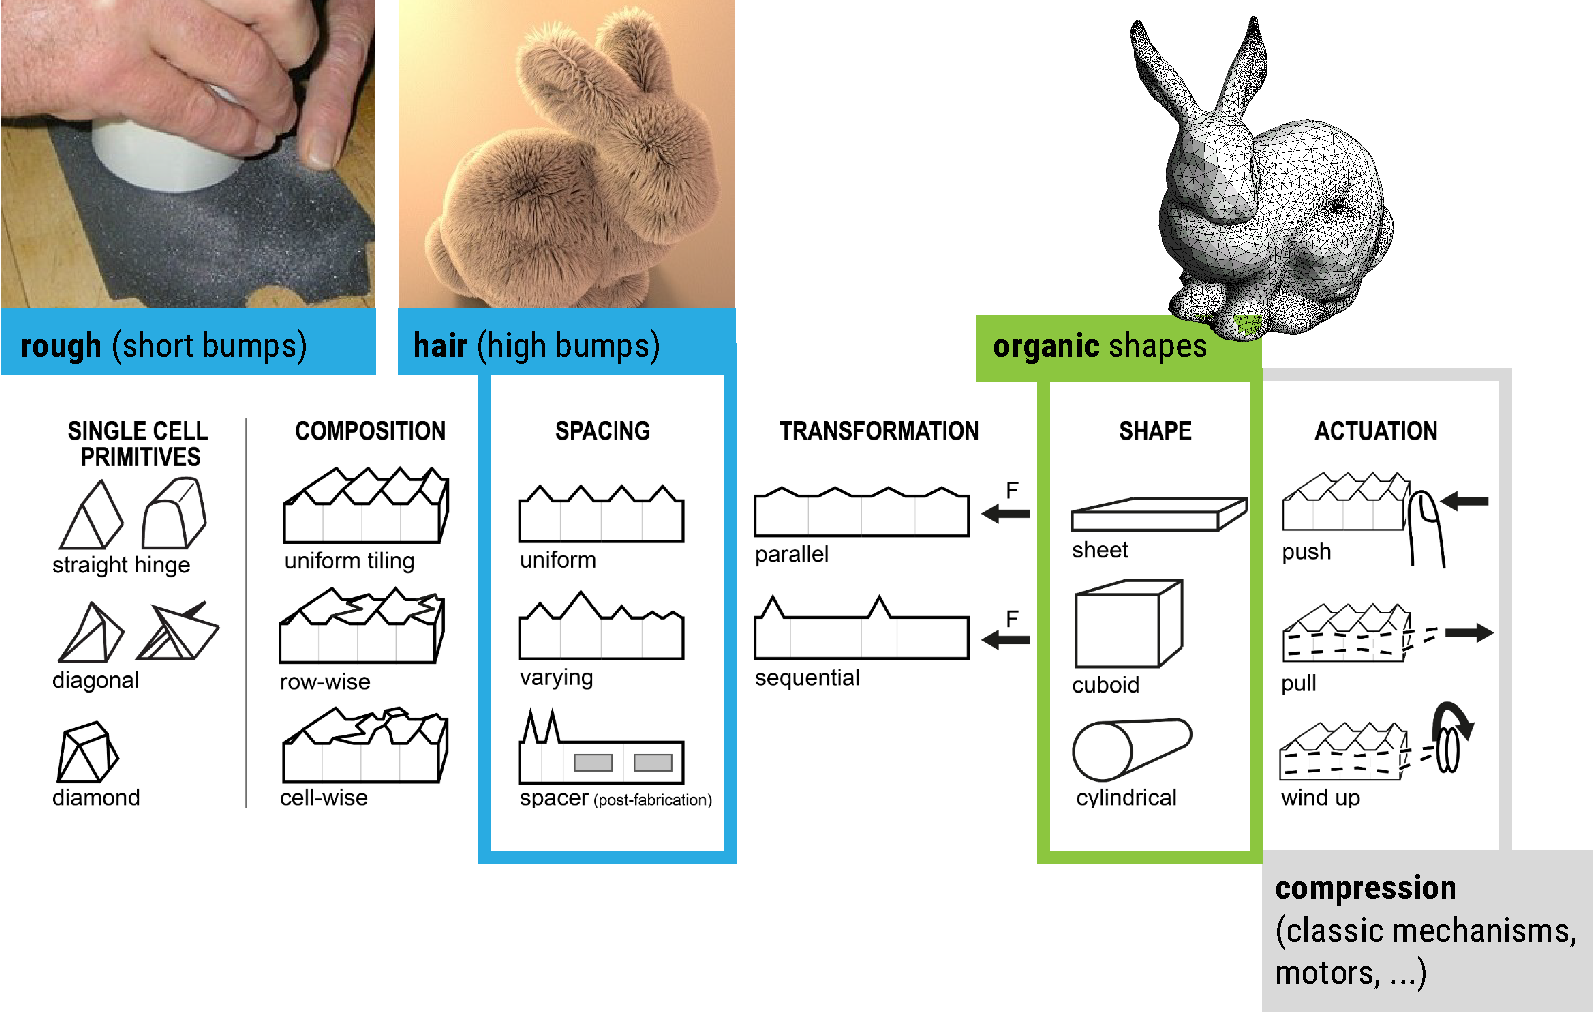
\includegraphics[width=\textwidth]{chapters/metamaterial-textures-FIG/18-discussion.pdf}
    \caption[Short figure name.]{Metamaterial textures can be actuated automatically (gray). In the future, our proposed cells should be extended to organic shapes (green). Using nano-scale printing could allow sophisticated textures such as fur or adaptable sandpaper (blue). 
    \label{fig:18-discussion}}
\end{figure}


\subsection{Limitations}

While we see this work as the first step towards creating textured objects using metamaterials, it certainly has a number of limitations. The most evident one is that our approach works only for objects in which exact dimensions are not critical. The exact length of a door handle, for example, is not critical for its functionality. In fact, our approach always generates a change in the object's overall shape. Secondly, our current approach is limited to actuation using a global force pulled along one dimension (e.g., when the user pulls the wires to configure the shoe sole). In the future, we want to investigate dynamic textures that can be actuated in two and three dimensions. Furthermore, we currently use external materials, such as the strings that are pulled, to actuate the metamaterial textures. In the future, we want to integrate the actuation with the metamaterial itself so that it can be fabricated in one piece. Lastly, our demonstration objects are limited in that the textures pop out on planes or cylindrical shapes only. Ideally, textures would be integrated in arbitrary organic shapes. 


\subsection{Alternative forms of actuation}

Since in this work, we explore the idea of materials that exhibit textures by means of metamaterials, we opted to actuate our textures in the simplest way (e.g., pushing, strings, etc.), so that no electronic components are required (such as motors, batteries, microcontrollers, etc.). However, alternative actuation mechanisms can certainly be used, e.g., motors, that will allow programmatic real-time behavior without users’ actions. For instance, one can envision how the door handle changes texture automatically by being digitally connected to the user's calendar.


\subsection{Outlook for nano-scale metamaterial textures}

The scale of our current textures was dictated by the resolution of our consumer-grade desktop printer. However, using state of the art high-resolution printers (e.g., nanoscribe\footnote{\url{http://www.nanoscribe.de/en/}}) it might be possible to uncover new opportunities using our approach. Firstly, by scaling down a design similar to that of Figure \ref{fig:9-amplitude-frequency}a, i.e., with long members that protrude a lot outside the object, it might be possible to use our approach to generate furry textures \cite{Laput2015, Ou2016a} that are transformable. 

Conversely, using high-resolution printers to fabricate cells with short members would yield a texture made from micro bumps that would feel ``rough" to the user. This could also be employed as a prototyping tool to alter an object’s friction when sliding on a surface or create adaptable sandpaper (Figure \ref{fig:18-discussion}, marked in blue).


\section{Conclusions}

We proposed an approach that leverages metamaterials to create transformable textures on 3D printed objects. We demonstrated the benefits of our approach in three objects and provided an interactive editor to allow researchers and users to create novel textures. 

We see metamaterial textures as a first step to integrate transforming textures into 3D printed objects. In the long run, we think such an approach might be relevant to disseminate more expressive haptics in everyday objects. We hope this opens new dialogs between UX and product designers and results in novel everyday objects with multiple pre-integrated textures that can be activated by the end user.


%Acknowledgements
%We want to thank David Lindlbauer for his insights in many discussions and Gierad Laput for his encouraging feedback.
